\section{Search Overview}
This section describes \sys's search algorithm and optimizations in greater detail.    

% The optimization algorithm takes a quality function, a language, and a dirty relation, and outputs a sequence of transformations (of max depth $k$) that maximizes the quality function.

\begin{algorithm}[t]
\KwData{Q, R, L, (k, $\gamma$)}

// Initialize priority queue of candidate programs\\
$P = \{NOOP\}$

\While{ $\exists ~ p \in P: \|o\| < k$ }
{
    \For{$p \in P: \|p\| < k$ }{
        
        Pop $p$ from the queue.
        
        \For{$t \in L$}{
             $p' = p \circ t$ 
             
             Push $p'$ with priority $\bar{Q}(p'(R))$.
        }
    }
    
    Pop all elements from with a priority greater than $\gamma$ times the lowest value in the queue.
}

\Return Lowest item on the queue
\caption{Greedy Best-First Tree Search}
\label{alg:main}
\end{algorithm}

\subsection{Naive Search Procedures}
In principle, any tree search algorithm over $L$ would be correct.
However, the traversal order and expansion policy is important in this search problem.  We describe the algorithmic and practical reasons why two naive procedures---breadth-first search (BFS) and depth-first search (DFS)---exhibit poor search runtimes.

\stitle{BFS} This approach extends each program in the search frontier with every possible data transformation in $\Sigma$.  To extend a candidate program $l_c$ with $T \in \Sigma$, it evaluates $Q((T\circ l_c)(R))$.  Unfortunately, the frontier grows exponentially with each iteration.  Additionally, evaluating every new candidate program $T\circ l_c$ can be expensive if the input relation is large.   Although the cost can be reduced by materializing $l_c(R)$, it is not possible to materialize all candidate programs in the frontier for all but the most trivial cleaning problems.    It is desirable to use asearch procedure that bounds the size of the frontier and the materialization costs.

% The first problem with this algorithm is that since each node in this tree $o$ represents a sequence of transformations.
% Evaluating the value of $o$ can be very expensive since it would have to evaluate the entire path to the root.
% $o$ is a composition of many transformations and may require a number of passes over the dataset.
% This can be avoided if we can materialize (either to disk or memory) the frontier,that is, for each node in the priority queue $o \in O$, we have a cached result of $o(R)$. 
% However, with BFS, the frontier is expoential in the support of the language and the system would quickly run out of memory.

\stitle{DFS} Depth-first search only needs to materialize the intermediate results for a single program at a time, however it is highly inefficient since the vast majority of programs that it explores will have low quality scores.  

\subsection{Basic Algorithm}
A best-first search expands the most promising nodes chosen according to a specified cost function.
We consider a greedy version of this algorithm, which removes nodes on the frontier that are more than $\gamma$ times worse than the current best solution.
Making $\gamma$ larger makes the algorithm asympotically consistent, whereas $\gamma=1$ is a pure greedy search.

The algorithm is described in Algorithm \ref{alg:main}.
The algorithm is initialized with an identity transformation. This identity transformation is placed on a priority queue where the priority is the aggregate quality after applying the transformation (in this case the quality of the original relation $R$).
Then, the algorithm ``expands'' all elements on the queue with description length of less than $k$.
By expansion, we mean that it removes the element from the queue composes the element with a transformation from the library.
Then, it places the new composed transformation onto the priority queue with its new quality score as the priority.
The algorithm then flushes the priority queue of all elements with priority more than $\gamma$ times worse than the current best solution.
This process repeats until all elements on the queue have a description length of $k$.

We can materialize (either to disk or memory) the frontier,that is, for each node in the priority queue $p \in P$, we have a cached result of $p(R)$. 
Then, when we expand the nodes to $p' = p \circ t$, we only have to incrementally evaluate $t(R)$.
After the node is expanded, the result is added to the cache if it within $\gamma$ of the best solution.
The basic algorithm described above is well-suited for this problem.
Without the greediness, the frontier might be exponentially large leading to an impractical amount of materialization.
By tuning $\gamma$, the user can essentially set how much memory is used for materialization.

\subsection{Optimizations Overview}

\stitle{Static Pruning} A static optimization is a regular expression that all transformation sequences must satisfy independent of the data. 
\[\textsf{static\_opt}(L, \text{regex} ) \mapsto L'\]
For example, since the find-and-replace operations are idempotent, i.e., $T(T(R)) = T(R)$, we may want to only consider the set of all sequences with no neighboring repeated transformations. Similarly, we may also want to prune all search branches that make no effect (i.e., find-and-replace New York with New York).
These two regular expressions alone reduce the overall number of evaluations by $48\%$ in the above example (120050 v.s. 226981 evaluations).
There are several other possible optimizations  such as avoiding changes that reverse previous changes $T_i(T_j(R)) = R$.


\stitle{Dynamic Pruning} A dynamic optimization can query the data and cost function to generate rules that are instance-specific:
\[\textsf{dyn\_opt}(Q, R, L) \mapsto \text{regex}\]
For example, we may want to ensure that all the evaluations are ``correlated'' with the cost function--that is it makes modifications that are likely to affect the costs.
This is possible if the cost separable where we have a score for each cell. In this case, we can find all the cells in violation of the functional dependencies and make sure that the ``source'' field of the find-and-replace operations only match values that are in violation.
These optimizations are called ``dynamic' because they can be determined from the active domain (i.e., after applying a transformation, recalculate new optimization rules).
Applying this optimization (in addition to the others) to the example reduces the search space to 1582 evaluations v.s. 226981 unoptimized (143x reduction).

\stitle{Parallelization}  Arbitrary constraint satisfaction problems are challenging because all variables can interact. While this is certainly the case for arbitrary quality functions, in many cases, data errors are localized. For example, replacing \texttt{San Francisc} with \texttt{San Francisco} has no effect on the records referring to \texttt{New York City}. The final class of optimizations are blocking rules which have been widely used in entity resolution systems:
\[\textsf{block}(Q, R, L) \mapsto \{R_1,...,R_k\} \]
For quality functions generated from dependencies, we can determine blocks analytically--looking at which violating tuples are linked through the constraint.
However, in general, these blocking rules can be learned (e.g., with clustering) or user defined.
The search can execute on each of the blocks independently.
\ewu{Emphasize that this is based on the decomposable nature of the quality function}

\stitle{Quality Estimation}  A large cost to the search algorithm stems from the need to execute the quality function over the output of each candidate program.  In some cases, it is possible to estimate the quality function without fully running the candidate program.  For instance, \ewu{foofah}.  Alternatively, it may be sufficient to run the candidate program over a sample of the input relation.  These are opportunities for future work.
\textbf{TODO}


\begin{figure*}
    \centering
    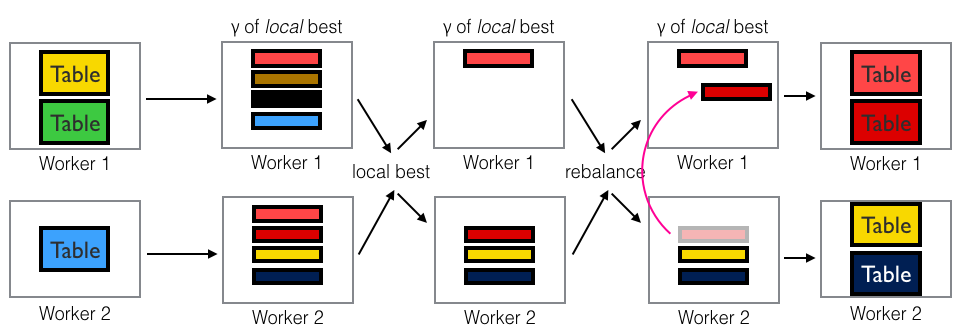
\includegraphics[width=0.6\textwidth]{figures/distributed.png}
    \caption{A schematic of the distributed search algorithm used to find a transformation sequence.    \label{fig:algo}}
\end{figure*}

\section{Search Optimizations}
\subsection{Parallelism}
The best-first search algorithm also is amenable to parallelization. One can parallelize over the two inner for loops $O \times L$. Each expansion can be forked into its own thread. However, this actually makes the materialization described above a bit more challenging. We use Ray~\footnote{https://github.com/ray-project/ray} to implement the parallel search. 

\subsubsection{Shared Memory Parallelization}
The most straight-forward case is when we have access to low-latency shared memory between the expansion threads. In each expansion round, the main thread will assign each expansion node to workers and they will evaluate a given transformation. Each worker will make a copy of $o(R)$ (the node it is expanding) into shared memory. 
If the expanded transformation is within $\gamma$ of the best current result, then it will update the copy, otherwise delete it. The point of synchronization is after all expansions are finished, and the main driver will flush all transformations less than $\gamma$ of the best result, and then assign new workers for the next round. 

\subsubsection{Distributed Parallelization}
In cases, where we do not have access to low-latency shared memory, the communication costs of the above algorithm can be impractical. For each expanded node, the entire table has to be communicated to each of the distributed nodes.
We consider a worker-driver model, and assume that the number of workers is $k$.
A schematic diagram of the algorithm is shown in figure \ref{fig:algo}.

\vspace{0.25em} \noindent  \textbf{Initialization. } 
Each worker has a copy of the base relation with no transformations.
In the first round of expansion, the driver assigns to each worker $\frac{|L|}{k}$ expansions. 
Each worker executes each of its assigned expansions, and stores the transformations that are within $\gamma$ of the best local result.

\vspace{0.25em} \noindent  \textbf{Reconciliation. }  Note that the global top-$\gamma$ set is a subset of the union of the all local results.
The workers then communicate the quality of their best transformation. This can be used to reconcile the local materializations to only the global top-$\gamma$ set.
This set is not necessarily balanced, e.g., one worker might have almost all of the top transformations.
The next step is a balancing step, where each worker communicates the number of materialized expansions it currently stores.
The workers with more than $\frac{|O|}{k}$ materialized expansions  randomly select ones to evict, and the driver re-distributes these to nodes with too few materialized expansions.
This is done by communicated the transformation and the result is re-computed on the new worker.
If $|O| < k$, then expansions are chosen at random to be replicated.
The result of the reconciliation step is that all workers have an evenly distributed set of materialized expansions.

\vspace{0.25em} \noindent  \textbf{Next Round. } After reconciliation, each worker is associated with a particular $o \in O$ (or a set of them). To parallelize, the driver must simply ensure that it assigns new expansions only to those workers that have materialized the parent.
The algorithm then repeats, expanding each node locally, and then reconciles the results.









\subsection{Learning Dynamic Pruning Rules}
To effectively search through the language of transformations, search heuristics are important.
However, it can be challenge to devise these heuristics \emph{a priori}.
This section describes how Machine Learning can be used to learn a search heuristic as data is cleaned.

\subsubsection{Motivation}
The search algorithms in  most automatic data cleaning frameworks are carefully tuned for a specific quality function or class of quality functions. For example, the chase used in functional dependency resolution does not make an edit to the table unless it enforces at least one tuple's FD relationship. Exploiting the structure of the specific problems allows for a tractable solution technique. Similarly, in entity matching problems, one restricts the search to only matching tuples that are likely to be similar based on some similarity metric.
These are not static optimizations, i.e., knowing how to prune the search space requires knowing the underlying data or making strong modeling assumptions about the types of transformations used.

\subsection{Algorithm \ewu{(Give a name?)}}
\sys executes the search on each block of data.
The result is a sequence of transformations to optimize the quality metric on that block.
Every transformation in this sequence can be treated as a positive training example $L^+$, and every transformation not in this sequence can be treated as a negative example $L^-$.
The idea is that if we apply the search to a sufficient number of blocks then we can train a classifier to predict whether a transformation will be included in the final sequence.
It is important to note that this prediction is over the transformations and not the data. 

Internally, \sys uses a Logistic Regression classifier to make this classification. The Logistic Regression is tuned towards False Positives (i.e., keep a bad search branch). This is done by training the model and shifting the prediction threshold until there are no False Negatives. 


\subsection{Requirements on Transformations}
Suppose we made only the following assumption about the language of transformations used.
Each transformation consists is described by a fixed-length feature vector in $\mathbb{R}^k$:
\[
\textsf{feat}: T \mapsto \mathbb{R}^k 
\]
An example of a featurization, consider a transformation from the the running example:
\begin{lstlisting}
find_replace(New York, New York City, city_name)
\end{lstlisting}
The featurization could encode the string similarity of the two literal parameters and an indicator vector describing which column it applies to.

Consider an alternative to a predefined search heuristic where we clean data in small blocks.
For the initial blocks, we search without a heuristic.
As we continuously perform the search, we train a classifier on these features to reject search branches that are not typically in the final solution.
This allows us to exploit any patterns in the literal parameters that repeatedly occur.

For example, some columns might not be dirty and are not worthwile to clean.
In the example above, another observation could be that the source and target strings in the optimal sequence are very close in terms of string similarity (as opposed to arbitrary transformations).
If each of these operations was featurized with a single scalar that is the edit-distance between the two strings, then the classifier could learn a pruning threshold (i.e., not considering find-and-replace operations above that threshold).


